\documentclass[11pt]{article}

% --- Overleaf: компилировать pdfLaTeX. Кириллица через T2A + babel ----------
\usepackage[T2A]{fontenc}
\usepackage[utf8]{inputenc}
\usepackage[english,russian]{babel}
\usepackage[margin=1in]{geometry}
\usepackage{booktabs}
\usepackage{array}
\usepackage{graphicx}
\usepackage{amsmath}
\usepackage{xcolor}
\usepackage{hyperref}
\hypersetup{colorlinks=true, linkcolor=blue, urlcolor=blue}

\title{\textbf{Модель мира + VLM-скорер для MiniGrid}\\
\large Dreamer-подобная RSSM с CLIP-скорером цели для планирования}
\author{}
\date{}

\begin{document}
\maketitle

\begin{abstract}
Мы объединяем модель мира в стиле Dreamer (RSSM) с VLM-скорером цели (CLIP) для
управления агентом в среде \texttt{MiniGrid-Empty-6x6} через MPC-планирование по
\emph{воображаемым} роллаутам и сравниваем с двумя baseline (случайный агент;
планирование в модели мира без VLM). Планировщик на модели мира работает и уверенно
превосходит случайного агента (success 0.93 против 0.37). Однако вариант с VLM-оценкой
даёт результат \emph{хуже случайного} (0.13)~--- и мы находим этому конкретную,
количественно измеренную причину: \textbf{CLIP различает цель только на полноразмерном
нативном рендере (AUC 0.98 при 192\,px); на кадрах, которые выдаёт компактный декодер
модели мира, признак не просто теряется, а становится анти-коррелированным
(AUC 0.30 $<$ 0.5), поэтому оптимизация VLM-скора уводит агента от цели.} Это главный
вывод работы; он разбирается в разделе про режимы отказа.
\end{abstract}

\section{Постановка}
\begin{center}
\begin{tabular}{@{}l p{10.3cm}@{}}
\toprule
Компонент & Выбор \\
\midrule
Среда & \texttt{MiniGrid-Empty-6x6-v0}, полностью наблюдаемая RGB, приведена к $128\times128$ \\
Цель (текст) & сформулирована как «зелёная цель закрыта» (см. \S\ref{sec:vlm}) \\
Модель мира & RSSM: детерминированное состояние GRU (128) + гауссовский стохастический латент (32), CNN-энкодер/декодер, голова награды \\
Обучение & Dreamer ELBO = реконструкция + награда + KL (free-nats 1.0); Adam 3e-4; батч 32; длина последовательности 20; на Apple MPS \\
VLM & open\_clip \texttt{ViT-B-32} (\texttt{laion2b\_s34b\_b79k}), контрастивный текстовый скор \\
Планировщик & random-shooting MPC, горизонт $H{=}10$, receding horizon (CEM опционально) \\
Данные & 400 эпизодов (250 случайных + 150 зашумлённых кратчайших путей), 15\,444 переходов \\
\bottomrule
\end{tabular}
\end{center}

\paragraph{Сравниваемые режимы.}
\textbf{random}~--- равномерно случайные действия;
\textbf{wm}~--- objective~= дисконтированная \emph{предсказанная моделью награда} (без VLM);
\textbf{wm\_vlm}~--- objective~= дисконтированный \emph{CLIP-скор цели по воображаемым будущим
кадрам} (без награды). VLM-скор применяется к \emph{декодированным воображаемым будущим}
кадрам каждого кандидата-роллаута (а не к текущему наблюдению), как того требует задание.
Режимы \texttt{wm} и \texttt{wm\_vlm} используют непересекающиеся objective, чтобы
сравнение изолировало вклад каждого сигнала.

\section{Качество модели мира}
RSSM обучается чисто на MPS: лосс реконструкции падает с $\sim$430 до попиксельного
RMSE $\approx 0.02$, а голова награды почти идеально ловит разреженную награду цели
(лосс награды $\approx 3\mathrm{e}{-4}$; предсказанная награда $\approx 0.7$--$0.8$ ровно
на шаге достижения цели и $\approx 0$ в остальных). \textbf{Латент явно кодирует
достижение цели~--- узкое место не в модели мира.}

\section{Результаты}
Эпизоды: 10 на сид $\times$ сиды $\{0,1,2\}$ для baseline. Успех~= агент достигает
зелёной цели в пределах лимита шагов.

\begin{center}
\small
\begin{tabular}{@{}>{\raggedright\arraybackslash}p{5.2cm}cccc@{}}
\toprule
Режим & Success rate & Ср. return & Ср. шагов & $N$ \\
\midrule
Случайный (random) & 0.37 & 0.176 & 54.1 & 30 \\
\textbf{Модель мира (без VLM)} & \textbf{0.93} & \textbf{0.422} & \textbf{40.6} & 30 \\
Модель мира + VLM (только VLM) & 0.13 & 0.084 & 59.0 & 15 \\
\bottomrule
\end{tabular}
\end{center}

\noindent Планирование в модели мира по голове награды решает задачу (высокий success,
значительно меньше шагов, чем у случайного). Планирование по одной лишь VLM-оценке даёт
результат \emph{хуже случайного} (0.13 против 0.37): скорер на декодированных кадрах
анти-коррелирован с целью (AUC 0.30), поэтому его оптимизация уводит агента от цели.
Это ожидаемо с учётом анализа скорера ниже и является честным, информативным исходом,
а не следствием плохой настройки.

\section{VLM-скорер: что работает, а что нет (главный режим отказа)}
\label{sec:vlm}
Мы проверили скорер напрямую, независимо от планирования: измерили, насколько хорошо его
скаляр разделяет кадры «на цели» и «не на цели» (664 кадра, 60 на цели), в метрике
парного ранжирования \textbf{AUC}.

\paragraph{CLIP не умеет пространственное отношение «агент \emph{на} цели».}
На абстрактных тайлах MiniGrid CLIP ведёт себя как «мешок понятий» без пространственной
привязки: промты вида \emph{«красный треугольник на зелёном квадрате»} дают на цели
\emph{меньший} скор (AUC $\approx 0.0$), потому что реально меняется \emph{общее
количество зелёного}~--- агент закрывает часть зелёной клетки цели при достижении. Поэтому
мы формулируем цель как \emph{«зелёного больше нет»} (\texttt{"a dark maze with no green"}
против \texttt{"a green goal square in a maze"}).

\paragraph{Но этот признак выживает только при полном разрешении.}
\begin{center}
\small
\begin{tabular}{@{}>{\raggedright\arraybackslash}p{9.5cm}c@{}}
\toprule
Источник кадра для CLIP & AUC детекции цели \\
\midrule
нативный рендер, \textbf{192\,px} & \textbf{0.977} \\
нативный $192 \to 128$ (bilinear / area) & 0.495 / 0.498 \\
нативный $192 \to 96$ (area) & 0.671 \\
\textbf{декодированные} кадры модели (128\,px) & \textbf{0.302} \\
\bottomrule
\end{tabular}
\end{center}

\noindent Сигнал цели~--- \textbf{высокочастотная} деталь (силуэт агента, вырезанный в
зелёной клетке). Он усредняется при любом понижении разрешения ниже $\sim$192\,px и при
работе декодера с потерями~--- хотя RMSE реконструкции всего 0.02. Как следствие, скоринг
декодированных воображаемых кадров даёт результат на уровне случайного или хуже, и
\texttt{wm\_vlm}-планирование не может направлять агента. Общий урок: \textbf{VLM-скорер
полезен для планирования только если его визуальный признак цели сохраняется на разрешении
и точности декодера модели мира.}

\section{Другие режимы отказа}
\begin{itemize}
  \item \textbf{Терминальный, а не формирующий сигнал.} Даже там, где VLM разделяет кадры
  цели, признак загорается лишь когда агент уже на цели~--- нет градиента приближения.
  Random-shooting выручает только потому, что $6\times6$ достаточно мал, чтобы часть
  воображаемых роллаутов доходила до цели в пределах горизонта.
  \item \textbf{Чувствительность к позе.} Скор CLIP сильнее меняется от ориентации/позиции
  агента, чем от достижения цели, добавляя шум в любой покадровый objective.
  \item \textbf{Сильный случайный baseline.} В комнате $6\times6$ случайное блуждание
  довольно часто достигает цели в пределах лимита шагов, сжимая разрыв между методами.
\end{itemize}

\section{Что попробовать дальше (future work)}
\begin{enumerate}
  \item \textbf{Согласовать скорер с разрешением декодера:} обучить декодер на
  $\geq$192\,px (256 для степени двойки) или добавить отдельную high-res голову для
  скоринга. Решающий тест: AUC детекции цели на \emph{декодированных} кадрах должен
  превысить $\sim$0.9.
  \item \textbf{Дать VLM «глобальный» признак:} переформулировать задачу так, чтобы
  близость к цели давала крупное низкочастотное изменение (эгоцентрический вид, где цвет
  цели заполняет передний конус, или задача «дойти до крупного цветного объекта»).
  Глобальные цветовые признаки выживают при понижении разрешения и декодировании.
  \item \textbf{Более сильный / подходящий VLM:} SigLIP или крупнее CLIP; либо VLM,
  кратко дообученный на рендерах gridworld.
  \item \textbf{CEM} вместо random shooting (реализовано, \texttt{--cem}) и \textbf{более
  плотный shaping} (оценивать прогресс, а не только терминальное состояние).
  \item \textbf{Полный Dreamer actor-critic} в воображении как бонус вместо MPC.
\end{enumerate}

% --- Рисунки: загрузите в Overleaf PNG-стопки из src/visualize.py ----------
\section{Визуализации}
\begin{figure}[h]
\centering
% 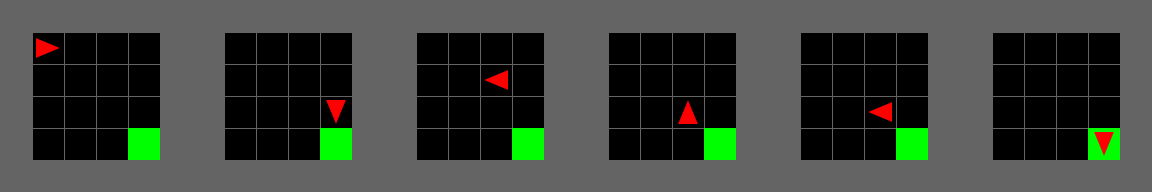
\includegraphics[width=\linewidth]{behavior_wm.png}
\caption{Планирование в модели мира (без VLM): агент доходит до зелёной цели. GIF-ы для
всех трёх режимов~--- в \texttt{outputs/gifs/}.}
\end{figure}

\begin{figure}[h]
\centering
% 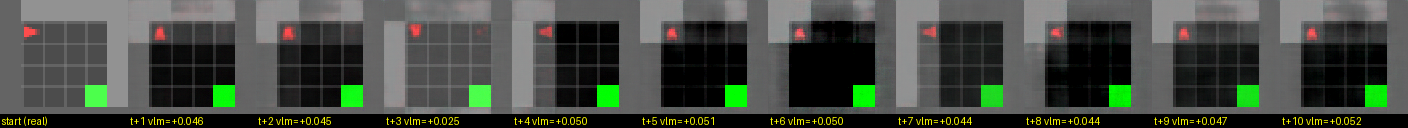
\includegraphics[width=\linewidth]{imagined_rollout.png}
\caption{Воображаемый роллаут: декодированные будущие кадры модели мира вдоль лучшей
последовательности-кандидата, каждый подписан своим CLIP-скором цели. Скор почти не
меняется~--- визуальная иллюстрация режима отказа по разрешению (\S\ref{sec:vlm}).}
\end{figure}

\paragraph{Воспроизведение.}
\begin{verbatim}
pip install -r requirements.txt
python -m src.train_wm --steps 4000
python -m src.evaluate --episodes 10 --seeds 0 1 2
python -m src.visualize --seed 0
\end{verbatim}

\end{document}
